% ms-syn-asyn - http://msdn.microsoft.com/en-us/library/windows/desktop/aa365683(v=vs.85).aspx


\section{Synchronous vs. Asynchronous I/O}
%What is B/NB I/O?
Server I/O can be handled either synchronously or asynchronously. A synchronous I/O operation is blocking, i.e., the thread that executes the current job is in a waiting state, where it does not compute anything, until it gets a response. An asynchronous I/O operation is non-blocking and therefore allows the thread to execute another job while waiting for the I/O operation to finish. This is illustrated on \Cref{fig:syncasync}. The figure does not show the overhead when using asynchronous I/O, which is causing this to not always be the best solution, especially if there are many short I/O operations \cite{ms-syn-asyn}.

\begin{figure}[H]
  \centering
  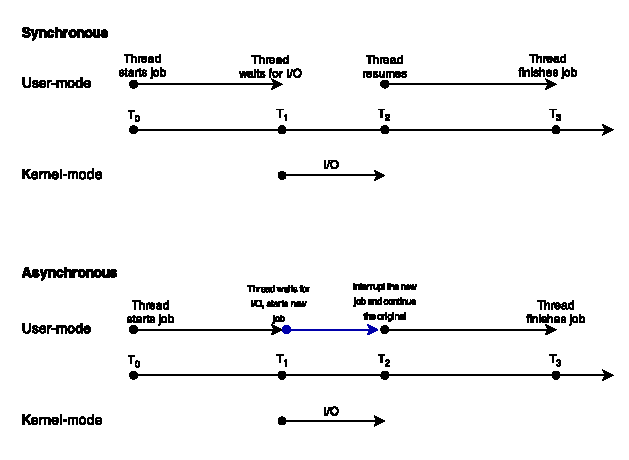
\includegraphics[scale=1.2]{billeder/sync-async.pdf}  
  \caption{Synchronous and asyncronous execution. Based on \cite{ms-syn-asyn}.}
  \label{fig:syncasync}
\end{figure}


The server I/O is implemented asynchronously, where the dispatcher asynchronously sends input to the correct game thread. Because of the %something something complicated app, hard to say 

%What are the advantages and disadvantages?

%Which alternative(s) is/are there?

%Why did we make the choice we did?

%How flexible is it?
% - Could it easily be changed? 
% - Could both be implemented and the framework-user decides which one to use?

\section{Synchronous vs. Asynchronous I/O}\fxfatal{This section will be rewritten with proper sources.}
For the client/server socket communication, a choice between synchronous and asynchronous I/O has to be taken.
% % blocking % %
Synchronous I/O can have a better performance than asynchronous, but can cause problems when using a threaded architecture that spawns a new thread for each client. This is particularly true when the server should be scalable in regards to its number of connected clients. There might be 5 and there might be 5000 or even more.
Tests show that threads are very efficient when it comes to memory and context switching, but only when the threads are kept alive for the entire execution of an application. This is not the case for our application, which will likely have many connections of varying durations during its up-time. \fixme{cite}\\\\
% % non-blocking % %
Asynchronous I/O is chosen for this project. It scales well when there are many clients, and the system should scale well with a potentially large number of clients. A notable advantage of asynchronous is that it limits the number of concurrent threads. The server asynchronously accepts a connection request from a client, and then starts an asynchronous worker thread to handle communication with the client. Meanwhile it continues to listen for new client connections.


%The ability to scale well does not come for free, however. Non-blocking IO is not always as fast as blocking IO and this can result in decreased performance. 